\chapter{Experiment Description}\label{sec:experiment}

\section{The Large Hadron Collider}
The Large Hadron Collider (LHC)~\cite{Evans_2008} is a high energy pp collider that serves several modern particle physics detector experiments. 
Built at CERN, straddling the French-Swiss border, and turned on for operation in 2008, it is the most powerful particle collider in history. 
The LHC was designed to collide protons at a maximum center of mass energy of $\sqrt s = 14\TeV$ 
with a maximum instantaneous luminosity of $10^{34}\cm^{-2}\mathrm{s}^{-1}$. To achieve this performance, the 27 km tunnel 
originally constructed for the Large Electron-Positron Collider (LEP)~\cite{Myers:226776} was repurposed to separately 
accelerate two counterrotating proton beams. The separate acceleration of the beams is made possible by oppositely oriented 
magnetic dipole fields in the two rings. When the beams achieve the desired energy, they are collided at one of four interaction points. 

The protons collided in the LHC are first gathered, bunched, and accelerated in other parts of the CERN accelerator complex before injection into the LHC ring. A detailed description of the injection chain can be found in Ref.~\cite{Benedikt:2004wm}, and a short summary is provided below. 
First, protons are stripped off of hydrogen atoms by a duoplasmatron and accelerated to 50\MeV by a linear accelerator (LINAC). Next, the protons are further accelerated 
in a series of synchroton rings of increasing size, the Proton Synchroton Booster (PSB), Proton Synchroton (PS), and Super Proton Synchroton (SPS). The SPS brings the 
proton beam energy up to 450\GeV. At this point, the beam is injected to the two LHC rings to be accelerated up to the final collision energy. Acceleration in the main 
ring is achieved by a system of thousands of superconducting dipole magnets, along with hundreds of correcting quadrupole magnets. A liquid helium cooling system is 
used to maintain the magnets at cryogenic temperatures. A full diagram of the CERN accelerator complex~\cite{CERN_complex}, including the parts relevant for the LHC, is shown in Fig. \ref{fig:accelerator_complex}.

\begin{figure}[tb]
  \centering
   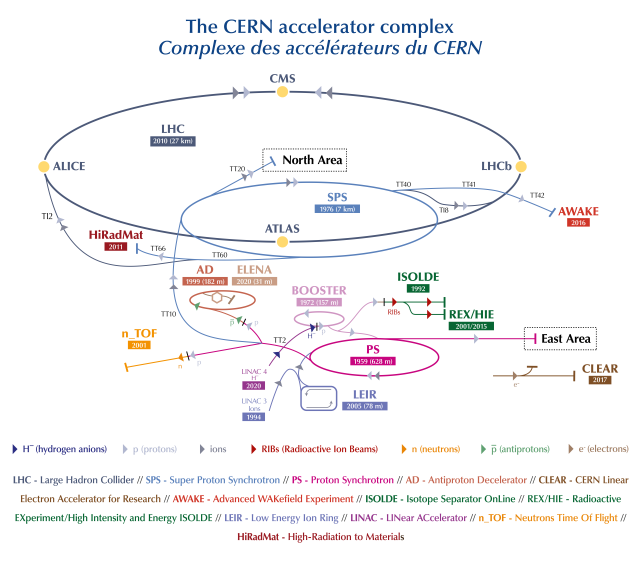
\includegraphics[width=0.9\textwidth]{fig/experiment/CCC-v2019-final-white.png}
	\caption[CERN accelerator complex.]{CERN accelerator complex~\cite{CERN_complex}.}
	\label{fig:accelerator_complex}
\end{figure}


\section{The Compact Muon Solenoid}
The CMS apparatus~\cite{CMS:2008xjf} is a multipurpose, nearly hermetic detector, designed to trigger on~\cite{CMS:2020cmk,CMS:2016ngn} and identify photons, electrons, muons, and (charged and neutral) hadrons~\cite{CMS:2015myp,CMS:2015xaf,CMS:2018rym,CMS:2014pgm}.
The central feature of the CMS apparatus is a superconducting solenoid of 6\unit{m} internal diameter, providing a magnetic field of $3.8$\unit{T}. Within the solenoid volume are a silicon pixel and strip tracker, a lead tungstate crystal electromagnetic calorimeter (ECAL), and a brass and scintillator hadron calorimeter (HCAL), each composed of a barrel and two endcap sections. The ECAL consists of 75,848 lead tungstate crystals, which provide coverage in pseudorapidity $\abs{\eta} < 1.48 $ in a barrel region (EB) and $1.48 < \abs{\eta} < 3.0$ in two endcap regions (EE). Preshower detectors consisting of two planes of silicon sensors interleaved with a total of $3$ radiation lengths of lead are located in front of each EE detector. Forward calorimeters extend the pseudorapidity coverage provided by the barrel and endcap detectors. Muons are measured in gas-ionization detectors embedded in the steel flux-return yoke outside the solenoid. Figure \ref{fig:detector} shows a schematic diagram of the CMS detector, and a more detailed description of the individual detector components and detector operation is provided below. 
%A more detailed description of the CMS detector, together with a definition of the coordinate system used and the relevant kinematic variables, can be found in Ref.~\cite{CMS:2008xjf}.

\begin{figure}[tb]
  \centering
   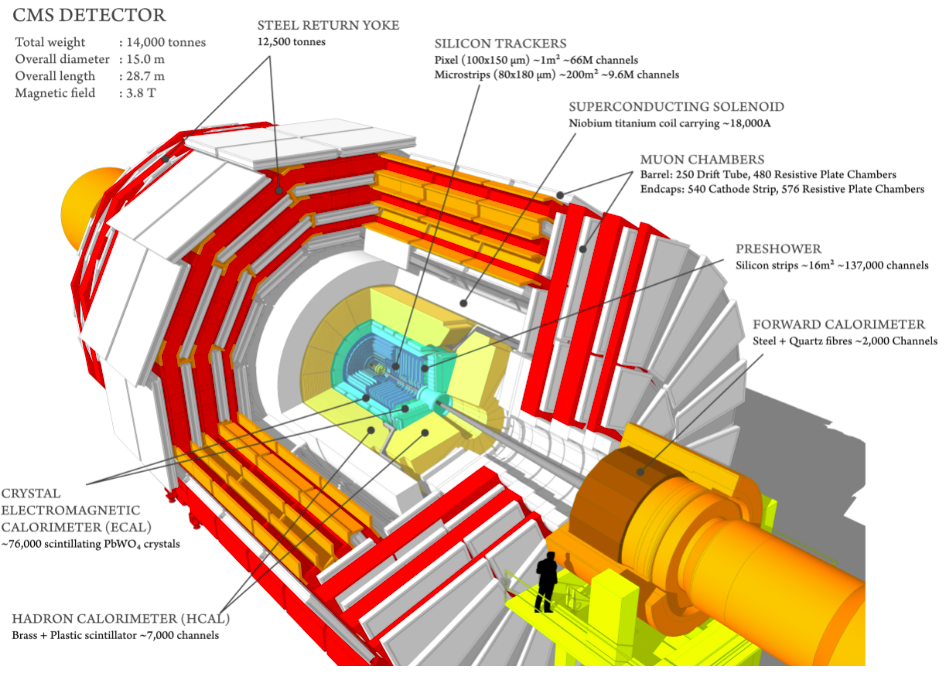
\includegraphics[width=0.75\textwidth]{fig/experiment/detector/cms_about_detector.png}
	\caption[CMS detector apparatus.]{CMS detector apparatus.~\cite{detector_image}}
	\label{fig:detector}
\end{figure}


\subsection{Superconducting Magnet}
The function of the superconducting magnet within the CMS detector is to bend the trajectories of charged particles. This is crucial for accurate particle identification and momentum measurement. 
Designed to provide a maximum magnetic field of $4$\unit{T}, its operating strength during pp collision runs is set to $3.8$\unit{T}. The bulk of the magnet is composed of NbTi, cooled by 
liquid helium to 4.5K, which is below the critical temperature for superconductivity. The magnet has a length of 12.5m, diameter of 6.3m, and mass of 220 tons. The solenoid encloses 
several detector components, including the tracker and the majority of the calorimeters. A steel flux-return yoke is built around the solenoid, and is composed of 5 wheels and two endcaps weighing 
a total of roughly 10,000 tons. 

\subsection{Inner Tracking System}
The inner tracking system is designed to reconstruct charged particle trajectories and vertices arising from particle decays. Comprised of a silicon pixel detector and silicon strip tracker, 
it covers the pseudorapidity region $|\eta| < 2.5$ and is designed for efficient and precise measurement of charged particles with transverse momentum (\pt) above about 1\GeV. 
At the LHC design luminosity for pp collisions, each bunch crossing leads to about 1,000 hits in the inner tracking system. As such, the inner tracking system was designed to be 
maximally radiation tolerant. 

The silicon pixel detector covers the inner region of $r < 10 \cm$. It is composed of $100 \times 150 \micron^{2}$ pixels, arranged in three barrel layers and two endcap disks. Due to the extreme 
radiation environment, the innermost layer was designed to be replaced after about two years of LHC operation. 
In response to LHC running conditions and detector degradation, a replacement and upgrade of the full pixel detector was made during the LHC extended year-end technical stop in 2016--2017. 

The silicon strip tracker covers the region $20 < r < 116 \cm$. It is divided into three subsystems: the Tracker Inner Barrel (TIB), Tracker Inner Disks (TID), and Tracker Outer Barrel (TOB). 
The strip thickness is $320 \micron$ ($500 \micron$) in the TIB/TID (TOB). A schematic diagram of the CMS inner tracking system in the r-z plane is shown in Fig. \ref{fig:cms_tracker}.

\begin{figure}[tb]
  \centering
   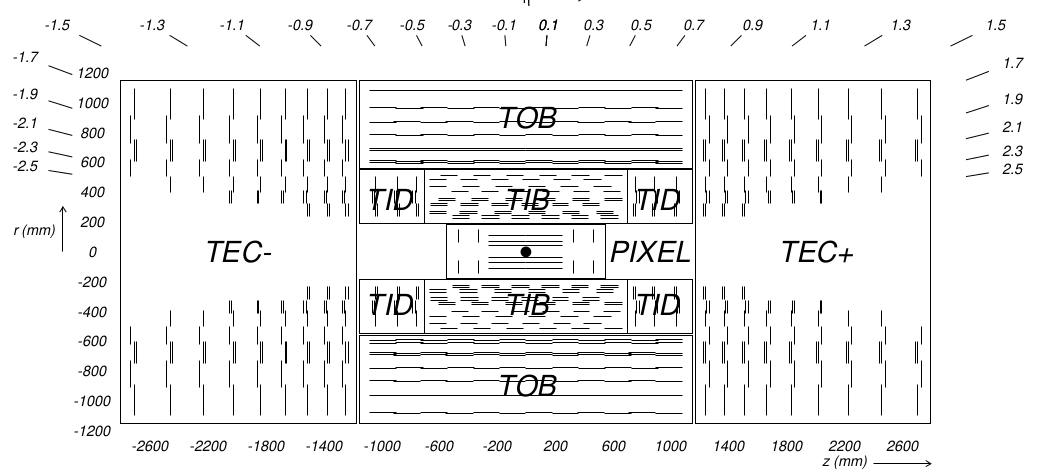
\includegraphics[width=0.8\textwidth]{fig/experiment/detector/cms_tracker.png}
	\caption[Cross section of the CMS inner tracking system in the r-z plane.]{Cross section of the CMS inner tracking system in the r-z plane.~\cite{CMS:2008xjf}}
	\label{fig:cms_tracker}
\end{figure}


\subsection{Electromagnetic Calorimeter (ECAL)}
The electromagnetic calorimeter (ECAL) is designed to identify and measure electromagnetic particles by inducing and characterizing electromagnetic showers. 
It is made up of 61,200 lead tungstate (PbWO$_4$) crystals in the barrel (EB), which covers $|\eta| < 1.479$, plus 7,324 crystals in each endcap (EE), which cover the range $1.479 < |\eta| < 3.0$. A preshower system lies in front of the EE. The preshower is a lead and silicon sampling calorimeter designed to aid in the identification of neutral pions and to improve the spatial resolution in the 
endcap region. 
The crystal length corresponds to 25.8 (24.7) radiation lengths in the EB (EE). When electromagnetic particles, such as 
electrons and photons, encounter the ECAL and interact with the crystal material, electromagnetic showers are induced. 
Light is emitted by the ECAL crystals proportional to the energy of constituent particles in the shower, allowing 
for reconstruction of the shower energy. An array of fast and radiation-tolerant photodetectors detects the emitted light, and this information is saved off detector. 
As shown in Fig. \ref{fig:cms_ecal_response}, the ECAL has maintained good performance with minimal degradation throughout the duration of Run 1 and Run 2 of the LHC.

\begin{figure}[tb]
  \centering
   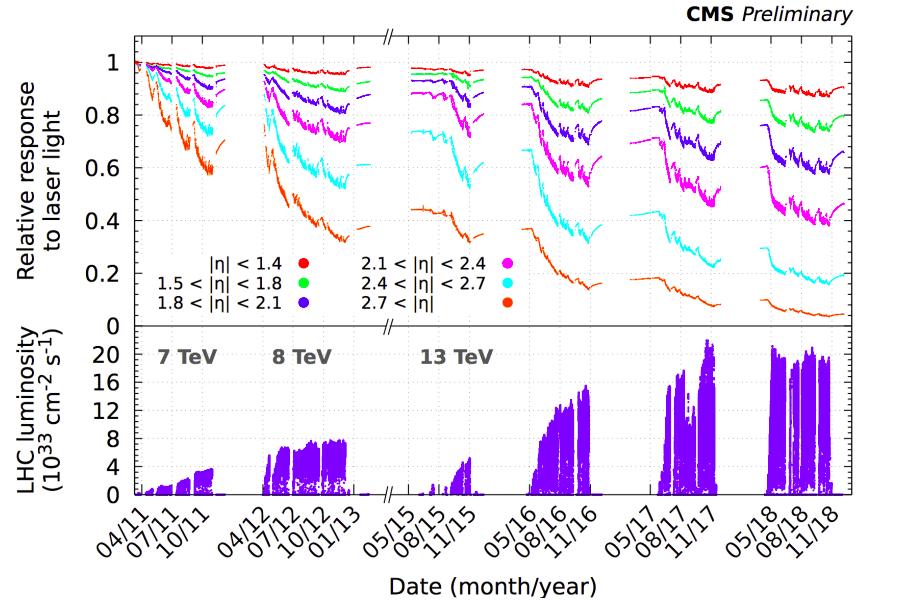
\includegraphics[width=0.8\textwidth]{fig/experiment/detector/cms_ecal_response.png}
	\caption[Response of the CMS ECAL crystals to injected laser light as a function of time, broken into regions of $|\eta|$.]
	{Response of the CMS ECAL crystals to injected laser light as a function of time, broken into regions of $|\eta|$~\cite{Cavallari:2798128}.}
	\label{fig:cms_ecal_response}
\end{figure}

\subsection{Hadronic Calorimeter (HCAL)}
Measurements of hadrons, jets, and missing transverse momentum are crucial at a hadron collider like the LHC. The CMS hadronic calorimeter (HCAL) is instrumental in such 
measurements. The HCAL is primarily a sampling calorimeter broken into several subdetectors. The barrel (HB) covers the range $|\eta| < 1.3$, the endcaps (HE) cover the range $1.3 < |\eta| < 3$, the forward calorimeter (HF) covers the range $3 < |\eta| < 5$, and an outer barrel calorimeter (HO) covers $|\eta| < 1.3$ outside of the solenoid magnet. 

Layers of brass absorber are interleaved with plastic scintillator in the HB and HE, with a total absorber thickness of 5.82--10.6 interaction lengths in the HB and about 10 interaction lengths in the HE. Scintillation light emitted by the active material is measured and transmitted off detector using hybrid photodiodes.
The design of the HF was motivated by the extreme particle fluxes in the very forward region. The HF is made up of steel plate absorbers, in which quartz fibers are inserted to serve as the active material. Cherenkov light is produced when shower particles moving at speeds above the Cherenkov threshold 
pass through the fibers, and a calculable fraction of the light is captured by the fibers. The function of the HO is to recover the energy in showers that leak through the HB, which is needed for the accurate measurement of missing transverse momentum. In the HO, the solenoid coil, itself, as well as a thick iron tail catcher, function 
as absorbers. This extends the effective HCAL depth to 11.8 interaction lengths everywhere except at the barrel-endcap boundary. 

\subsection{Muon Detectors}
The CMS muon detector system is comprised of a set of gas ionization detectors embedded in the flux-return yoke outside the solenoid magnet. 
These detectors cover the range $|\eta| < 2.4$. The positioning of the muon detectors outside the magnet takes advantage of the fact that muons deposit minimal energy in the detector 
materials within the solenoid, such as the calorimeters. Most other types of particles will have deposited their energy before reaching the muon system, so using the combination of muon detector and tracker information, CMS is able to reconstruct muons with good momentum resolution. The gas ionization detectors in the muon system come in three types: drift tubes (DTs), cathode strip chambers (CSCs), and 
resistive plate chambers (RPCs). The DTs cover the barrel region ($|\eta| < 1.2$) and are arranged in four stations, each with 60--70 drift chambers containing a gas mixture of 85\% Ar and 15\% CO$_2$.
The CSCs are multiwire proportional chambers composed of anode wire planes interleaved with cathode panels. Muons passing through the CSCs ionize a gas mixture of 40\% Ar, 50\% CO$_2$, and 10\% CF$_4$, 
and the electrons flow to the anodes, yielding a detectable avalanche of charge. Covering the region $|\eta| < 2.1$, the RPCs are composed of oppositely charged parallel plates enclosing a gas mixture 
of primarily $\mathrm{C}_2\mathrm{H}_2\mathrm{F}_4$. One advantage of the RPCs is their good time resolution, which is less than the LHC bunch spacing time of 25 ns. This makes them useful for fast muon triggering that matches
muon tracks to the relevant bunch crossing. Figure \ref{fig:muon_system} shows a cross-sectional view of the CMS detector highlighting the muon system components. 

\begin{figure}[tb]
  \centering
   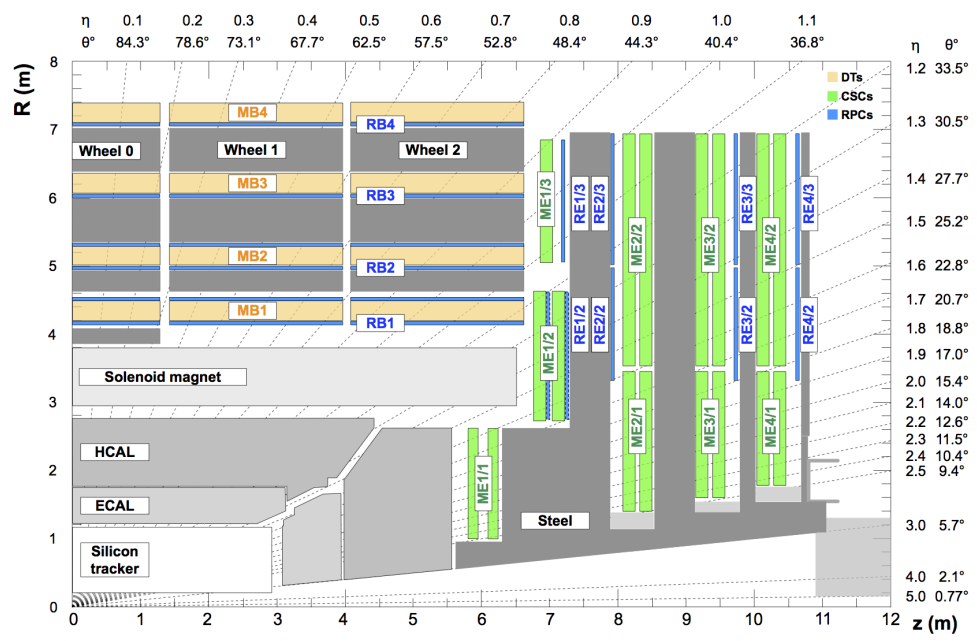
\includegraphics[width=0.9\textwidth]{fig/experiment/detector/muon_sys_r-z.png}
	\caption[Diagram of the CMS detector in the r-z plane showing the components of the muon system.]
	{Diagram of the CMS detector in the r-z plane showing the components of the muon system~\cite{CMS:2008xjf}.}
	\label{fig:muon_system}
\end{figure}

\section{Trigger System}
At the LHC, the proton beam crossing interval is 25 ns, which corresponds to a pp collision rate of 40 MHz. Recording the full set of detector information for each collision is unfeasible, as there is far too much data to save to disk. Because of this, the CMS experiment employs a two-tiered trigger system, designed to preserve information of physics interest while reducing the 
stored event rate to a more manageable 100 Hz. The first level of the trigger (L1) is a hardware trigger, which reduces the event rate from 40 MHz to about 100 kHz. The second layer is the 
high level trigger (HLT), a processor farm using software optimized for fast processing. 

The L1 trigger is implemented using field-programmable gate arrays and application-specific integrated circuits, and has local, regional, and global components. First, local patterns in the calorimeters, track segments, and hit patterns in the muon chambers 
are processed by the Trigger Primitive Generators (TPGs). The TPGs rank and sort primitive objects corresponding to particle candidates based on energy, momentum, and reconstruction quality. Information
from the TPGs is taken as input by regional triggers for the calorimeters and muon systems. These regional triggers further determine candidate physics objects, as well as energy sums and isolation
information. Finally, this information is fed to a set of global triggers, which rank trigger objects across the entire detector. The final global trigger must decide whether to accept or 
reject an event based on information input from the global calorimeter and muon trigger systems. Algorithms used for this decision can be based on single object \pt thresholds and multiplicity-related 
requirements, such as the presence of multiple jets, among other criteria. Events passing the L1 trigger are read out and passed to the HLT for further processing. 

In contrast to the L1 trigger, the HLT incorporates the full physics object reconstruction based on the full precision of the detector. This allows the HLT to accept and reject events with algorithms 
of similar quality to those used by offline analyses. Over 13,000 central processing unit cores are dedicated to HLT processing. For speed and efficiency, reconstruction and filtering algorithms are applied in increasing order of complexity. If a filter sequence fails, the rest of the reconstruction is skipped. Additionally, processing is done regionally based on the L1 candidates and relevant detector components 
passed as input to the HLT. Events that pass the HLT are assigned to relevant data streams based on their physics content. For the \hzg{} search, the relevant streams are the Double Muon and 
Double Electron streams, triggered by events with two muons or two electrons passing a set of minimum \pt requirements and other cuts. 

\section{Object Reconstruction}
The global event reconstruction (also called particle-flow (PF) event reconstruction~\cite{CMS:2017yfk}) aims to reconstruct and identify each individual particle in an event, with an optimized combination of all subdetector information. In this process, the identification of the particle type (photon, electron, muon, charged hadron, neutral hadron) plays an important role in the determination of the particle direction and energy. Figure \ref{fig:particles_interact} provides a simple visualization of how each type of particle types interacts with each of the CMS subdetectors. An overview of the reconstruction procedure for each particle type is provided below.

\begin{figure}[tb]
  \centering
   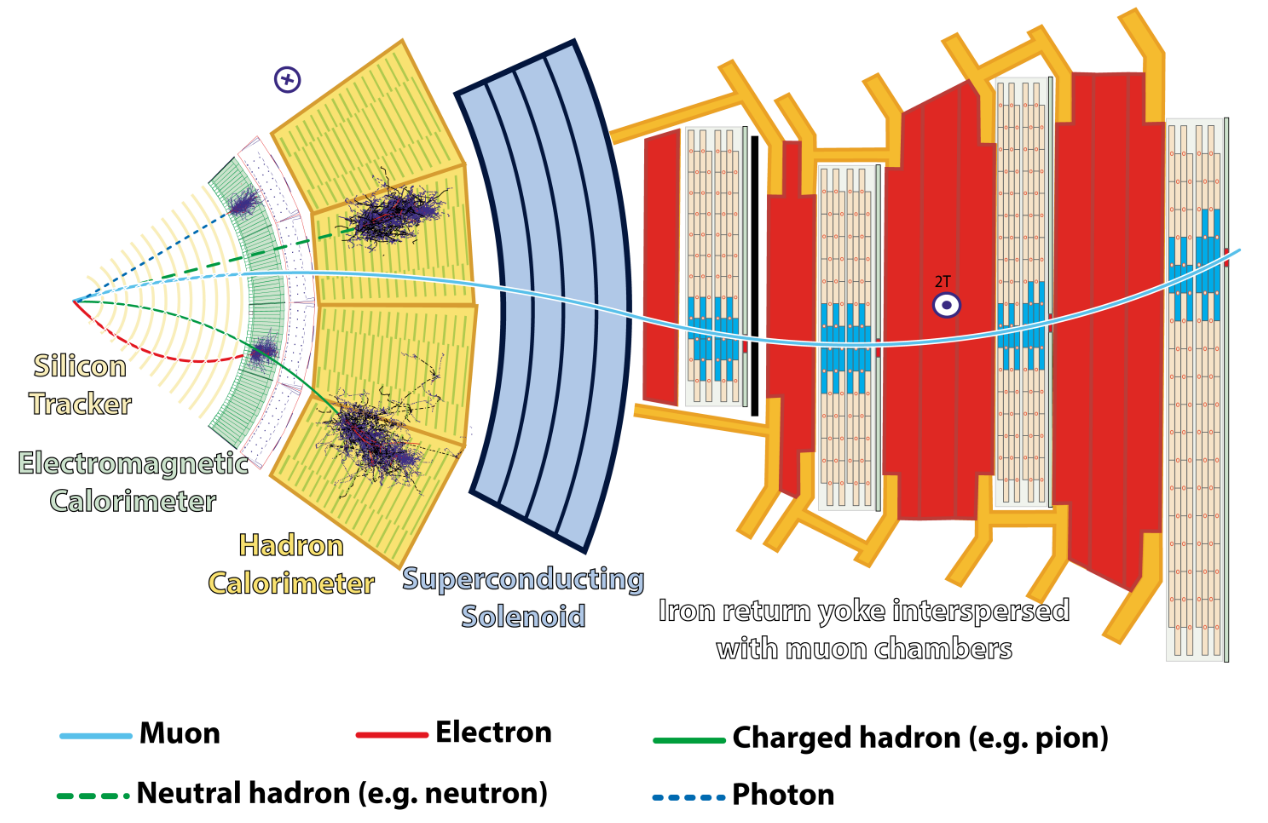
\includegraphics[width=0.9\textwidth]{fig/experiment/reconstruction/cms_detector.png}
	\caption{Visualization of different types of particles interacting with the CMS detector.}
	\label{fig:particles_interact}
\end{figure}

\subsection{Photon and Electron Reconstruction}
Photons and electrons interact with the material in the ECAL, depositing the majority of their energy before reaching the HCAL. As they interact, photons convert into 
electron-positron pairs and electrons radiate bremsstrahlung photons. This leads to the formation of an electromagnetic shower. Because of this, the original particle energy 
is split into multiple energy deposits, which must be combined to reconstruct the original energy. Deposits in individual ECAL crystals are combined into clusters, 
and these clusters are in turn combined into superclusters. Two algorithms are used to define superclusters: the ``mustache" algorithm, and the ``refined" algorithm.
The mustache algorithm defines a seed cluster with energy above a certain threshold, and then combines it with other clusters within a region of the $\eta$-$\phi$ plane centered at the 
seed location. The refined algorithm uses the mustache superclusters and tracking information to extrapolate bremsstrahlung and conversion tracks, in order to decide whether a cluster should belong 
to the supercluster. 

The distinction between photons and electrons is made using tracking information, where photons are associated with no tracks and electrons with tracks. The Gaussian Sum Filter (GSF)~\cite{Adam:815410} track 
fitting algorithm is used to identify and characterize tracks that might be associated with an electron. It first begins with a hit pattern in the tracker, which is used as a seed. This seed 
can either be tracker-driven, coming from the collection of generic tracks tested for mutual compatibility, or it can be ECAL-driven, where a mustache supercluster is compared in location with 
a collection of tracker hit patterns to determine if the supercluster is consistent with the trajectory indicated by the track. Electron seeds are then converted into reconstructed electron tracks. 
In the absence of any GSF electron tracks, a photon candidate is obtained. Additional distinction between photons and electrons is obtained through further selection requirements. 
Fig. \ref{fig:electron_resolution} shows the energy resolution for simulated electrons in the barrel and endcaps as a function of generated \pt. 
The measured energy resolution for electrons produced in $\PZ$ boson decays in  $\Pp\Pp$ collision data ranges from $2$--$5$\%, depending on electron pseudorapidity and energy loss through bremsstrahlung in the detector material~\cite{CMS:2020uim}.

\begin{figure}[tb]
  \centering
   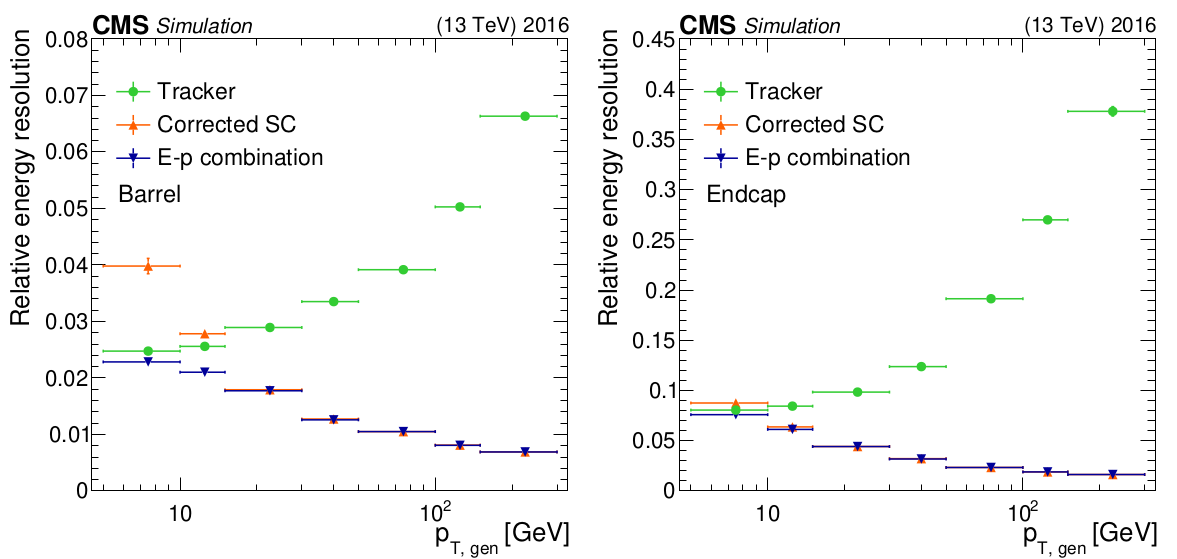
\includegraphics[width=0.8\textwidth]{fig/experiment/reconstruction/electron_resolution.png}
	\caption
	[Energy resolution for simulated electrons in the barrel (left) and endcaps (right) as a function of generated \pt. The green markers represent tracker measurement only, the orange markers represent ECAL measurement only, and the purple markers represent the combination of tracker and ECAL information.]
	{Energy resolution for simulated electrons in the barrel (left) and endcaps (right) as a function of generated \pt~\cite{CMS:2020uim}. The green markers represent tracker measurement only, the orange markers represent ECAL measurement only, and the purple markers represent the combination of tracker and ECAL information.}
	\label{fig:electron_resolution}
\end{figure}

\subsection{Muon Reconstruction}
Muon reconstruction utilizes information from the muon detectors and the tracker. First, detector hits in the CSCs, DTs, and RPCs are used to build standalone tracks using a Kalman filter~\cite{FRUHWIRTH1987444} technique.
Subsequently, these standalone muon tracks are combined with tracker information via two algorithms. So-called ``tracker muons" are reconstructed using an ``inside-out" algorithm, which starts from 
tracker tracks and matches them to DT or CSC segments. So-called ``global muons" are reconstructed with an ``outside-in" approach, which starts from standalone muon tracks and matches them 
to tracker tracks using a Kalman filter technique. If both algorithms reconstruct a muon sharing the same tracker track, the two outputs are merged into a single muon candidate.
In general, the tracker muon algorithm is more efficient for low muon \pt, while the global algorithm is more efficient for high \pt. 

The momentum of muons is obtained from the corresponding track momentum. Matching muons to tracks measured in the silicon tracker results in a \pt resolution, for muons with \pt up to $100$\GeV, of $1$\% in the barrel and $3$\% in the endcaps. The \pt resolution in the barrel is better than $7$\% for muons with \pt up to $1$\TeV~\cite{CMS:2018rym}. As shown in Fig. \ref{fig:muon_resolution}, this corresponds to a dimuon mass resolution in $\PZ\to\mpmm$ events of roughly 1--2\GeV, depending on the pseudorapidity of the muons~\cite{MUON:DP2019}. 

\begin{figure}[tb]
  \centering
   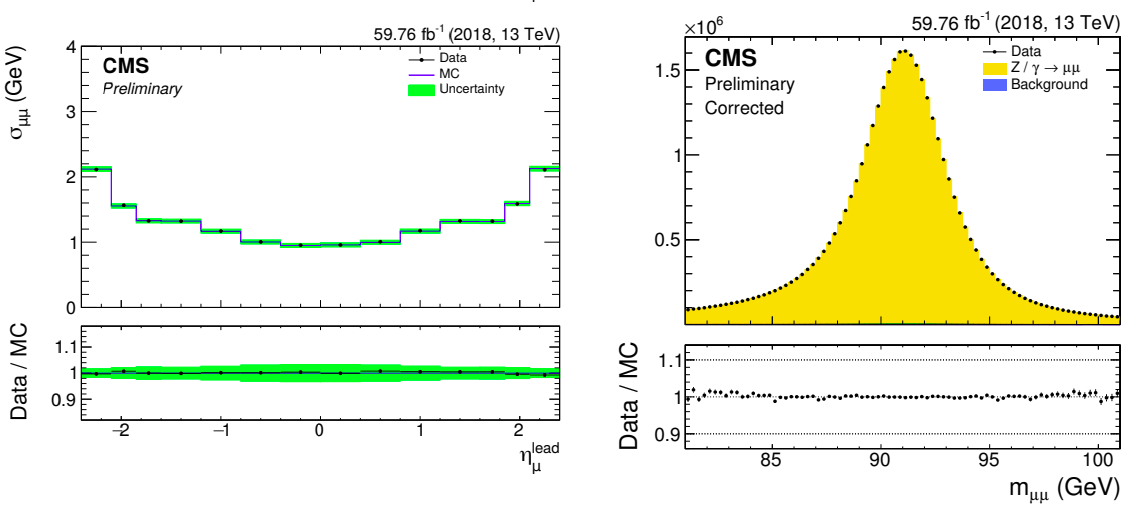
\includegraphics[width=0.9\textwidth]{fig/experiment/reconstruction/muon_resolution.png}
	\caption
	[Left: dimuon mass resolution as a function of leading muon $\eta$ for $\PZ\to\mpmm$ events in 2018 data and simulation. Right: reconstructed dimuon mass.]
	{Left: dimuon mass resolution as a function of leading muon $\eta$ for $\PZ\to\mpmm$ events in 2018 data and simulation. Right: reconstructed dimuon mass.~\cite{MUON:DP2019}}
	\label{fig:muon_resolution}
\end{figure}


\subsection{Hadron Reconstruction}
All particles within an event that are not reconstructed as photons, electrons, or muons are reconstructed as hadrons. Note that within the tracker acceptance ($|\eta|<2.5$), all ECAL clusters 
not linked to a track are considered photons. All of the remaining ECAL and HCAL clusters are processed further by the PF algorithm. The HCAL clusters are 
first linked to any associated tracks and ECAL clusters. Then, a comparison is made between the calorimetric energy sum and the sum of the track momenta. If the calorimetric energy sum is 
compatible with the sum of track momenta, a charged hadron is reconstructed. If the calorimetric energy sum is greater than the sum of track momenta, the excess prompts the reconstruction of photons and neutral hadrons, depending on the size of the excess. 

\subsection{Jet Reconstruction}
For each event, hadronic jets are reconstructed as clusters of PF particles, including photons, electrons, muons, and hadrons. For clustering, the infrared and collinear-safe anti-\kt algorithm~\cite{Cacciari:2008gp, Cacciari:2011ma} is used. The goal of jet clustering algorithms is to combine PF particles together into a single jet object by merging them together based on their relative geometric distances and transverse momenta (\kt). In the case of the anti-\kt algorithm, clustering proceeds from smallest geometric distance to largest, weighted by squared inverse \kt. This inverse weighting 
preferentially combines PF particles with higher momenta before lower momenta, for a given distance. The advantage of this approach is that low momentum particles are more likely to be clustered 
with high momentum counterparts, rather than with other low momentum particles. It follows that these low momentum particles will not significantly modify the jet shape, whereas the more important, high-momentum particles, will. A precise definition of the anti-\kt algorithm is given in equation \ref{eq:antikt}. 

\begin{equation}
	d_{ij} = min(k_{T,i}^{2p}, k_{T,j}^{2p})\frac{(\eta_i - \eta_j)^2 + (\phi_i - \phi_j)^2}{R^2},\;\; d_i = k_{T,i}^{2p}
	\label{eq:antikt}
\end{equation}

The indices i and j refer to two PF particles, the parameter $p$ is taken to be -1, and the radius parameter $R$ can be tuned. For standard jets in CMS, as used in this analysis, $R$ is set to 0.4. Particles are clustered from smallest $d_{ij}$ to largest, until there is no $d_{ij}$ smaller than $k_{ti}^{-2}$, at which point the final jet is defined. A visual representation of the anti-\kt algorithm is shown in Fig. \ref{fig:anti_kt_diagram}.

\begin{figure}
  \centering
   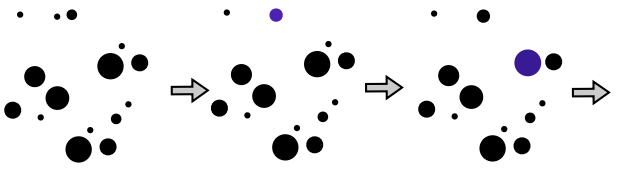
\includegraphics[width=0.9\textwidth]{fig/experiment/reconstruction/jet_clustering.png}
	\caption{An example of the first few steps of the anti-\kt jet clustering algorithm.}
	\label{fig:anti_kt_diagram}
\end{figure}

Jet momentum is determined as the vectorial sum of all particle momenta in the jet, and is found from simulation to be, on average, within $5$--$10$\% of the true momentum over the entire \pt spectrum and detector acceptance. Additional $\Pp\Pp$ interactions within the same or nearby bunch crossings (pileup) can contribute additional tracks and calorimetric energy depositions to the jet momentum. To mitigate this effect, charged particles identified as originating from pileup vertices are discarded, and an offset correction is applied to correct for the remaining contributions~\cite{CMS:2020ebo}. The jet energy resolution, as shown in Fig. \ref{fig:jet_resolution}, typically amounts to $15$--$20$\% at $30$\GeV, $10$\% at $100$\GeV, and $5$\% at $1$\TeV~\cite{CMS:2016lmd}.

\begin{figure}
  \centering
   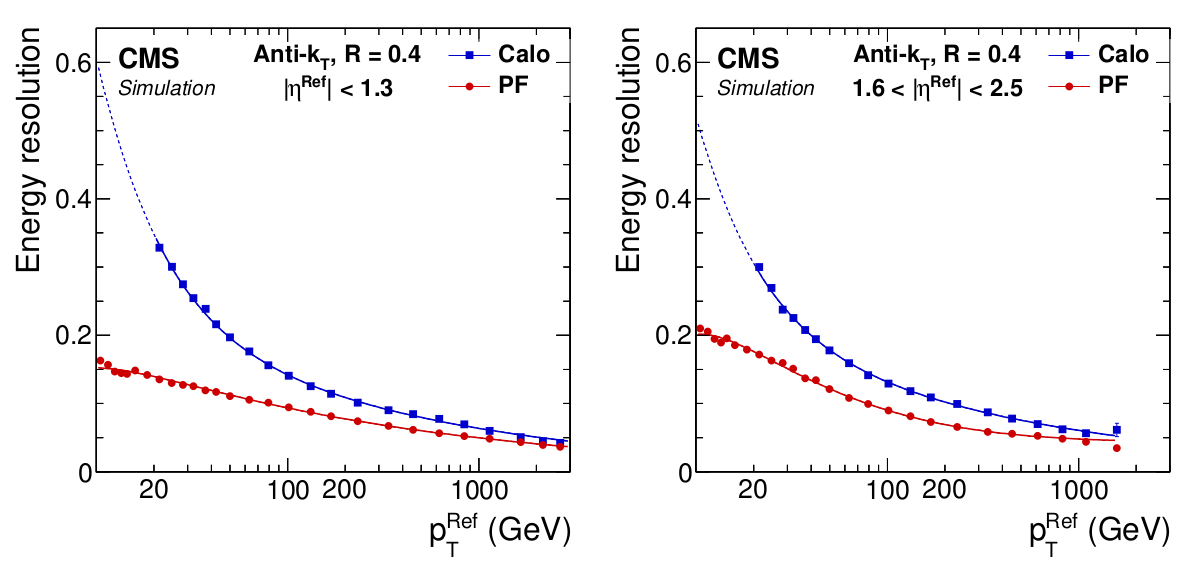
\includegraphics[width=0.9\textwidth]{fig/experiment/reconstruction/jet_energy_resolution.png}
	\caption
	[Jet energy resolution as a function of simulated jet \pt in the barrel (left) and in the endcap (right) regions. Calo refers to the sum of ECAL and HCAL energy deposits, 
	while PF corresponds to jets clustered from PF particles using the anti-\kt algorithm.]
	{Jet energy resolution as a function of simulated jet \pt in the barrel (left) and in the endcap (right) regions~\cite{CMS:2017yfk}. Calo refers to the sum of ECAL and HCAL energy deposits, 
	while PF corresponds to jets clustered from PF particles using the anti-\kt algorithm.}
	\label{fig:jet_resolution}
\end{figure}

